\begin{figure}[t]
	\centering
	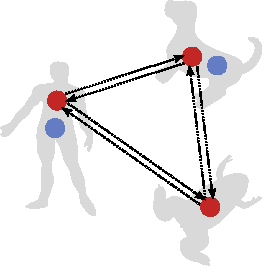
\includegraphics[width=0.4\textwidth]{img/triangulation-bbh.pdf}
	\caption[Triangulation of bidirectional best hits]{
		Bidirectional best hit (BBH) triangulation. To identify genes as orthologous
		in the presence of potential gene loss or incomplete data, they must be BBH
		in three species.  In this example, the red gene fulfills this criterion.
		The blue gene cannot be unambiguously identified as orthologous, as it is
		not present in the frog and paralogy is possible (compare to
		\autoref{fig:graph-based-strat}).  Graphic modified from
		\citet{altenhoff2012}.
	}
	\label{fig:triangulation-bbh}
\end{figure}
